\section{Формулировка предлагаемого решения}

\begin{figure}[ht]
\center{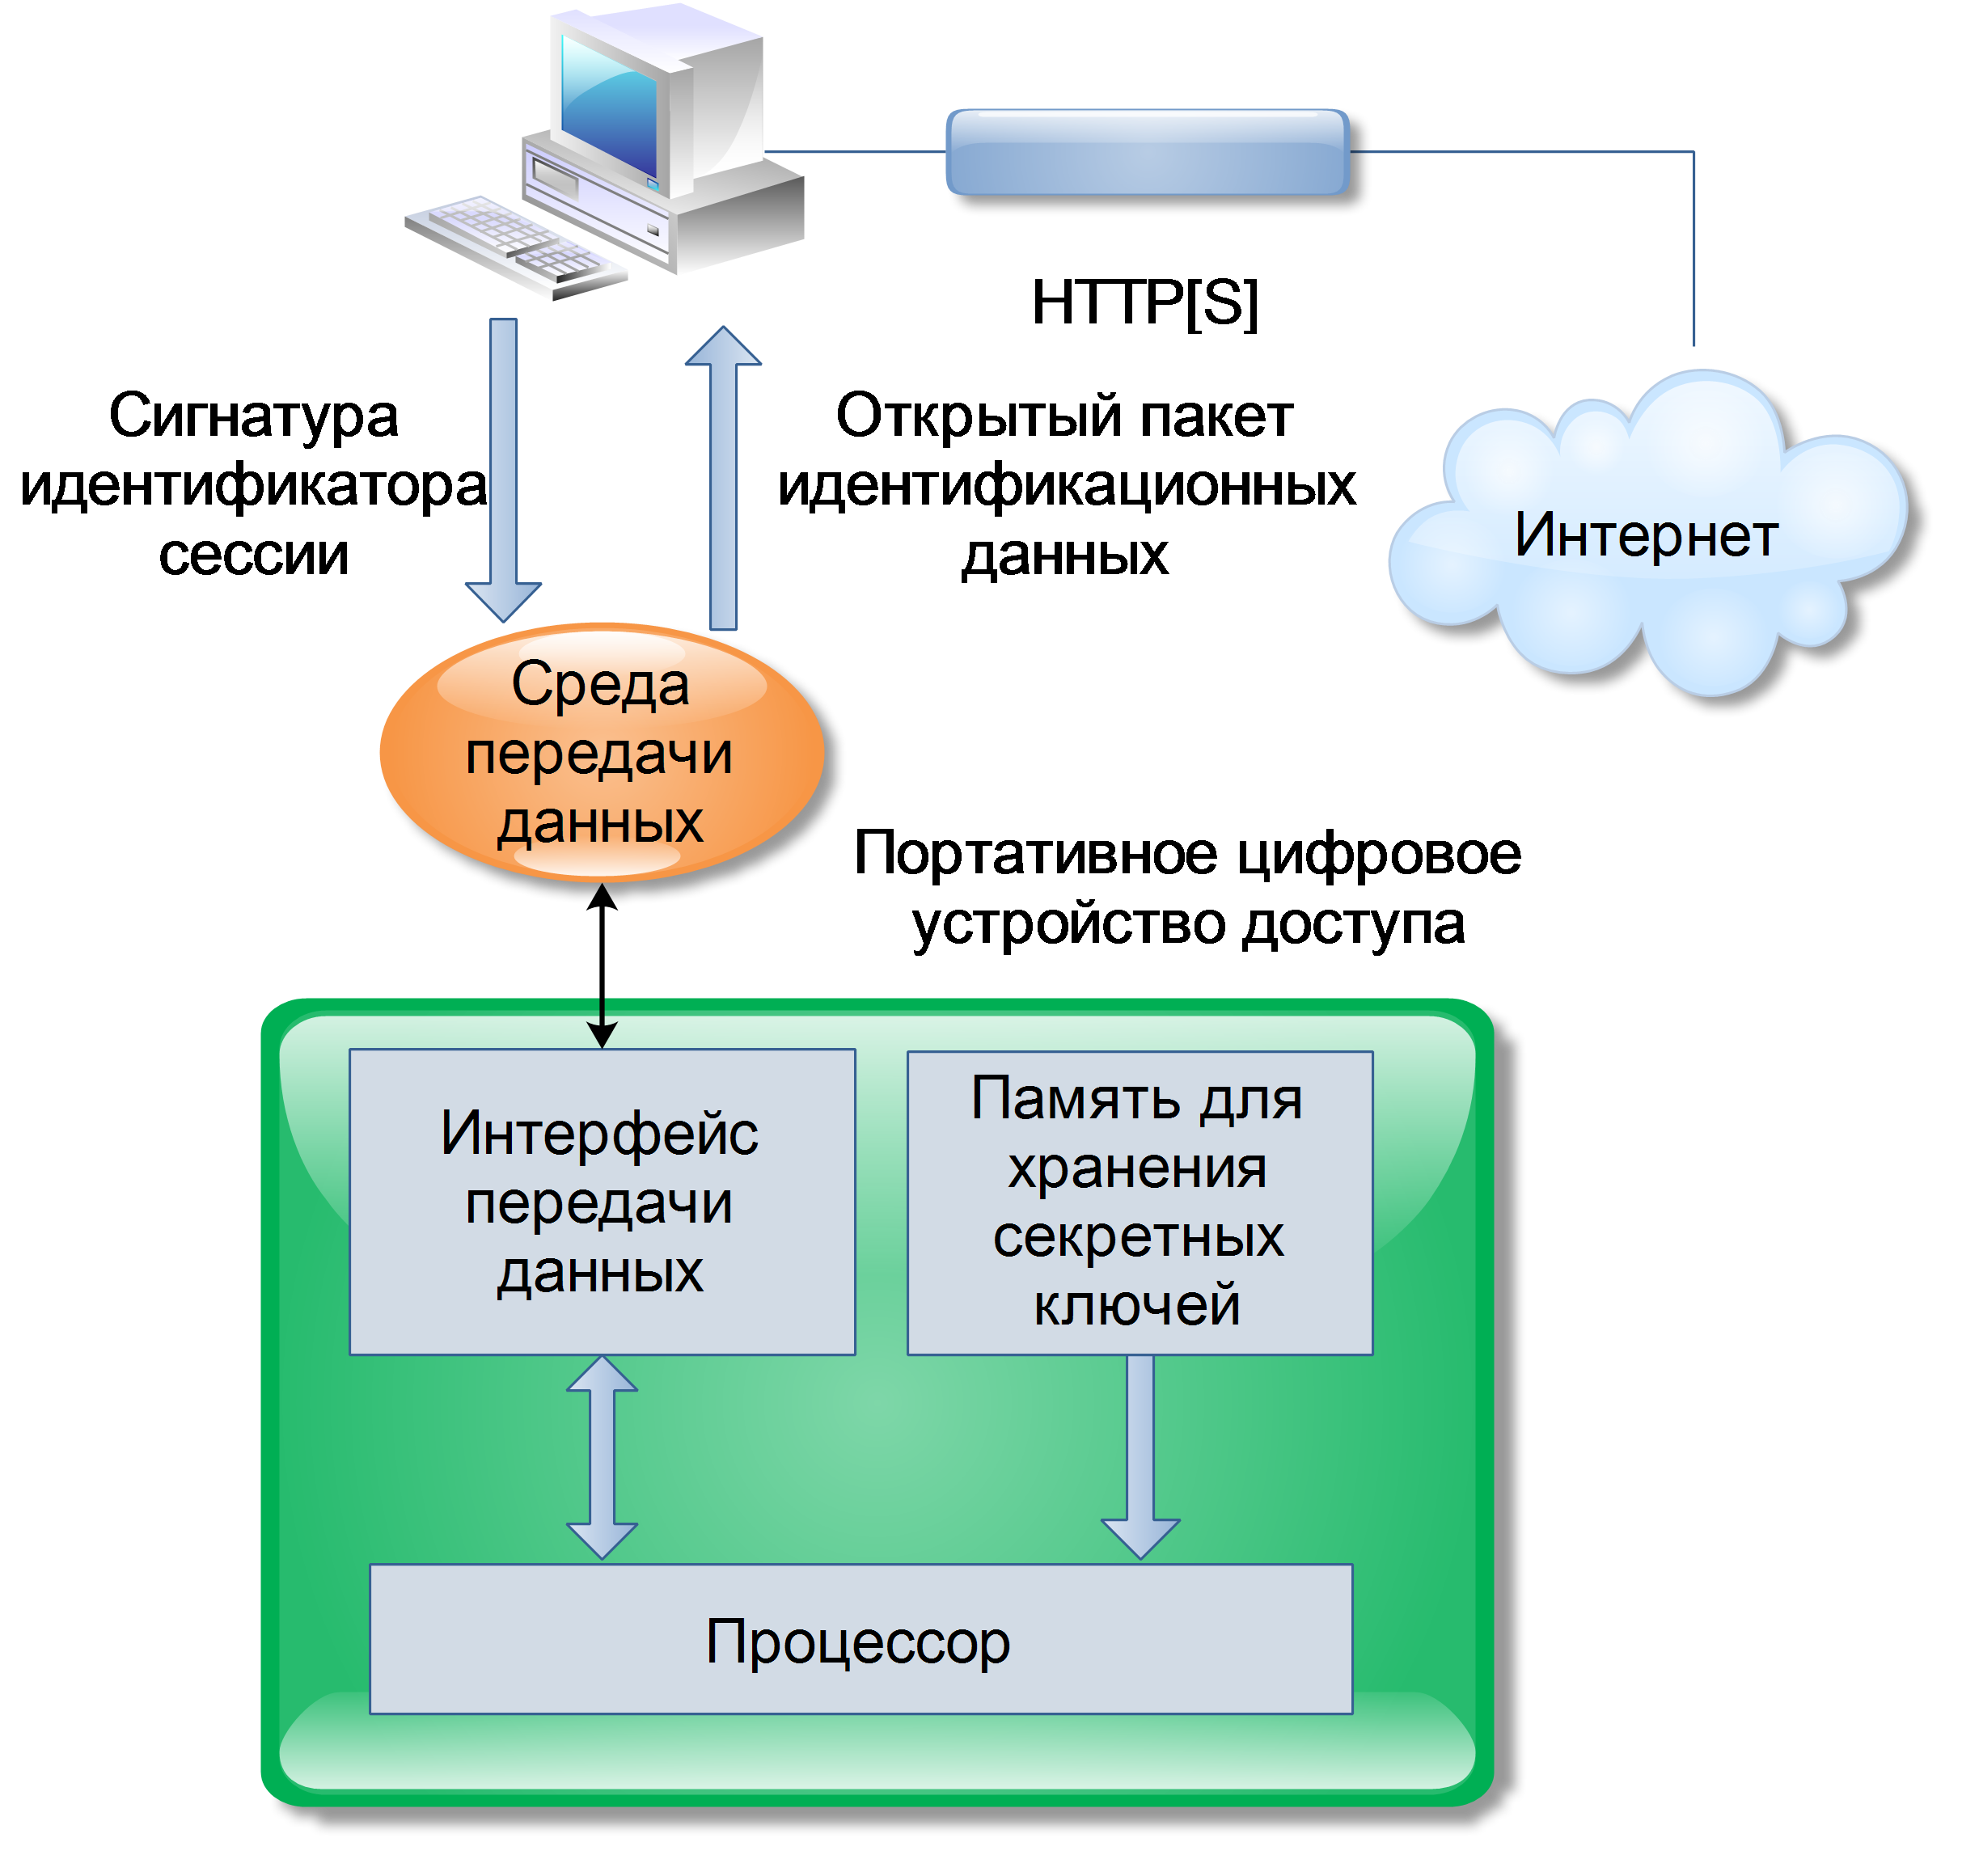
\includegraphics[width=0.7\linewidth]{1-5-1}}
\caption{Концептуальная схема подсистемы аутентификации пользователей}
\label{ris:1.5.1}
\end{figure} 

На основе данных, полученных в результате анализа, можно сформулировать вариант
решения, который позволит устранить недостатки существующих систем доступа.

Исходя из указанных недостатков традиционных подходов к аутентификации, была
предложена новая идея, основанная на использовании портативного
электронного устройства в качестве инструмента доступа к Web-порталу. Процесс
доступа основывается на реализации алгоритмов шифрования.
~\cite{thesis_digit_sign,thesis_smart_card}

Уникальность данной разработки заключается в том, что доступ осуществляется при
помощи специального устройства, способного не только хранить секретные ключи, но
и на их основе вычислять параметры алгоритмов, которые могут далее передаваться
в открытом виде.

Таким образом мастер-ключ алгоритма не копируется на персональный компьютер, где
он сильно уязвим и может быть подвержен атаке. Считывание ключей из устройства
физически неосуществимо в силу ряда принципов работы микроконтроллера, на основе
которого оно построено. Выходные данные алгоритма вычисляются на устройстве и
далее передаются по открытым каналам.

Данное устройство должно быть изготовлено таким образом, чтобы оно соединялось с
персональным компьютером с помощью стандартного интерфейса передачи данных (USB)
без использования дополнительных считывателей. Концептуальная схема данной
технологии представлена на рисунке~\ref{ris:1.5.1}.

Таким образом, с помощью данного устройства достигается механизм двухфакторной
аутентификации. Кроме того, данное устройство можно использовать для
осуществления электронного документооборота применяя технологию
электронно-цифровой подписи.

В качестве области приложения данный программно-аппаратный комплекс можно
рассмотреть в контексте системы управления доступом к распределеной сети
корпоративных порталов.~\cite{conf_itnop_lsa_concept}

\begin{figure}[ht]
\center{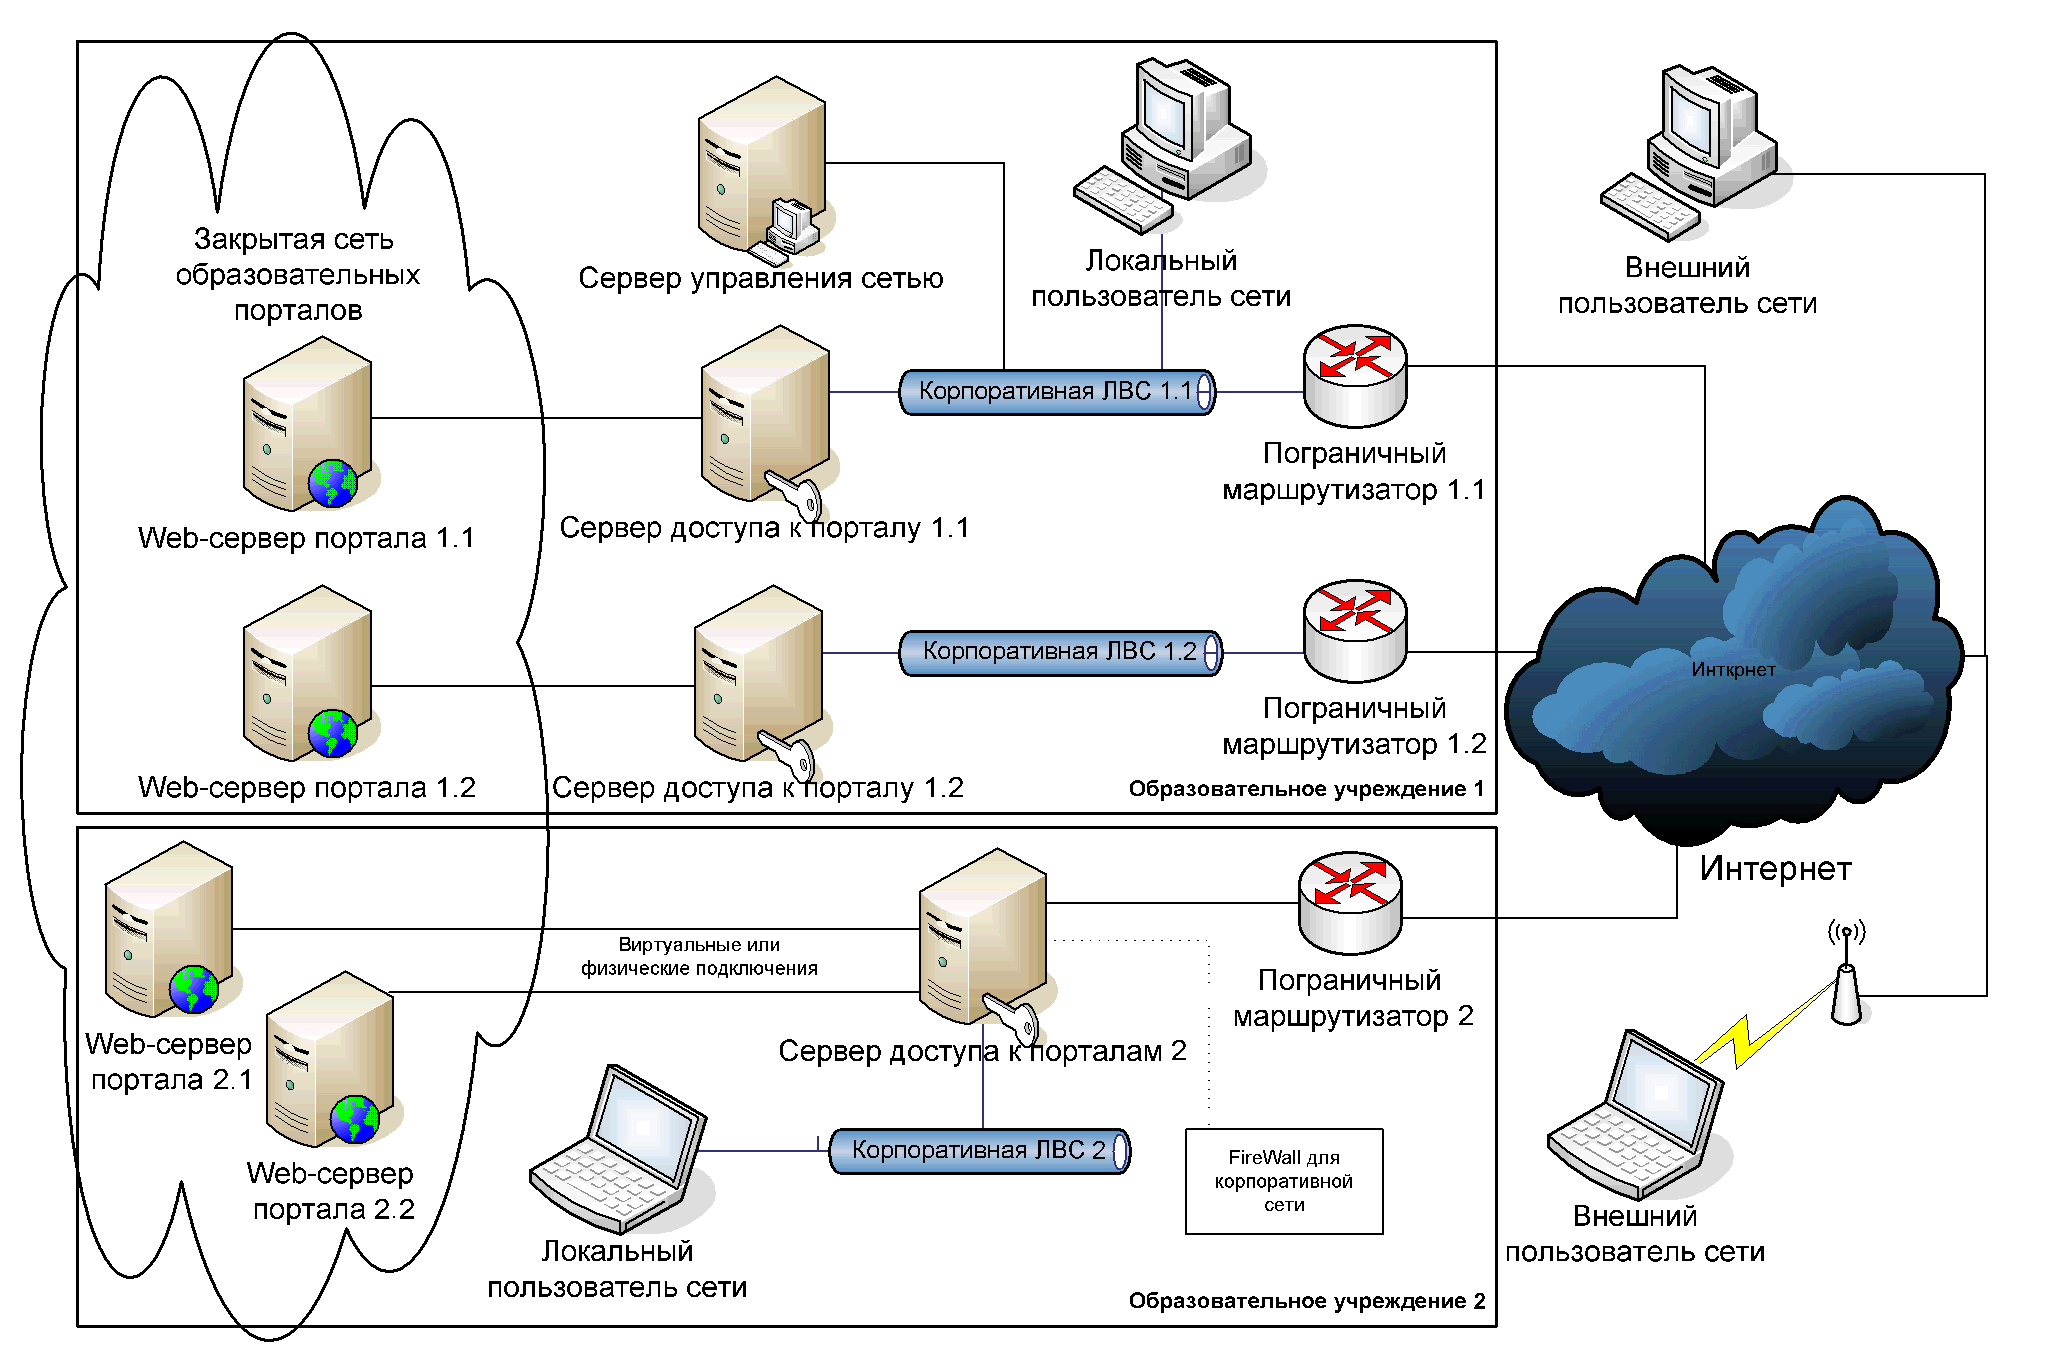
\includegraphics[width=1\linewidth]{1-5-2}}
\caption{Схема развертывания элементов распределенной системы доступа}
\label{ris:1.5.2}
\end{figure} 

Программно-аппаратный комплекс доступа на основе портативных
электронных цифровых ключей предполагает наличие серверной и клиентской части.
Серверная часть представляет собой наборы алгоритмов, которые производят
верификацию сгенерированных шифров со стороны пользователя. Клиентская часть в
свою очередь состоит непосредственно из портативного цифрового устройства
доступа и web-скриптов, загружающихся в браузер клиента через web-страницу и
осуществляющих взаимодействие с ключом.

В результате интеграции в систему управления доступом (беря во внимание схему
на рисунке~\ref{ris:1.5.2}) серверная часть инсталлируется на сервера доступа.
Портативное цифровое устройство доступа подключается к пользовательской машине. Во время
работы устройства синхронизирующие программы подгружаются через web-страницу с
сервера доступа и выполняют информационный обмен с ключом. Таким образом можно
осуществлять аутентификацию пользователя в системе и производить электронный
документооборот, используя электронно-цифровую подпись (ЭЦП).